
\documentclass[tikz,border=10pt]{standalone}

\usepackage{verbatim}
\usetikzlibrary{arrows,intersections}

\begin{document}
	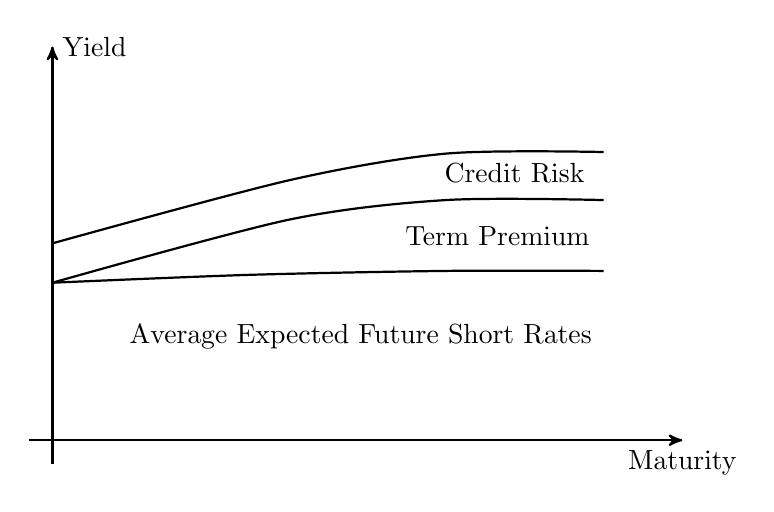
\begin{tikzpicture}[
	thick,
	>=stealth',
	dot/.style = {
		draw,
		fill = white,
		circle,
		inner sep = 0pt,
		minimum size = 4pt
	}
	]
	\coordinate (O) at (0,0);
	\draw[->] (-0.3,0) -- (8,0) coordinate[label = {below:Maturity}] (xmax);
	\draw[->] (0,-0.3) -- (0,5) coordinate[label = {right:Yield}] (ymax);
	\draw plot[smooth] coordinates {(0,2.5) (3,3.3) (5,3.64) (7,3.66)};
	\draw plot[smooth] coordinates {(0,2) (3,2.8) (5,3.05) (7,3.05)};
	\draw plot[smooth] coordinates {(0,2) (2.5,2.1) (5,2.15) (7,2.15)};
	\draw (4.85,3.65) node[below right] {Credit Risk};
	\draw (4.35,2.85) node[below right] {Term Premium};
	\draw (0.85,1.6) node[below right] {Average Expected Future Short Rates};
	
%	\draw plot[smooth] coordinates {(0,2) (3,3) (5,3.55) (7,3.6)};
%	\draw plot[smooth] coordinates {(0,1.5) (3,2.3) (5,2.8) (7,2.8)};
%	\draw plot[smooth] coordinates {(0,1.5) (3,1.6) (5,1.7) (7,1.8)};
%	\draw (5,3.5) node[below right] {Credit Risk};
%	\draw (4.5,2.5) node[below right] {Term Premium};
%	\draw (0.85,1.1) node[below right] {Average Expected Future Short Rates};
	\end{tikzpicture}
\end{document}